\chapter{System Testing and Evaluation}\label{chap:testingEvaluation}

\section{Graphical user interface testing}
\begin{figure}[ht]
\subsubsection{Table 28: user interface testing}
\centering
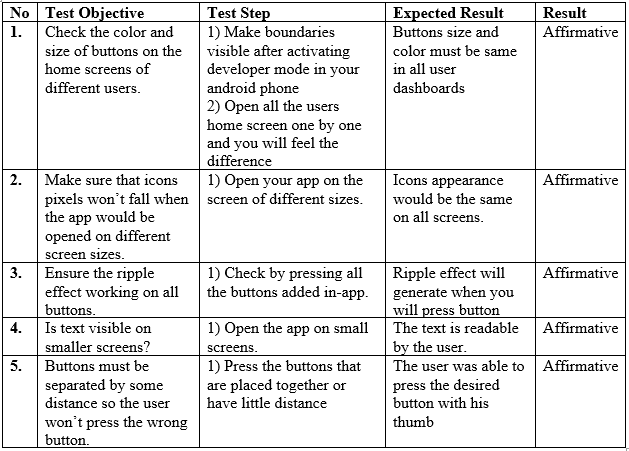
\includegraphics[width=0.8\textwidth]{UITesting1}
\captionof{table}{User Interface Testing}
\end{figure}

\section{Graphical user interface testing}
\begin{figure}[ht]
\subsubsection{Usability testing}
\centering
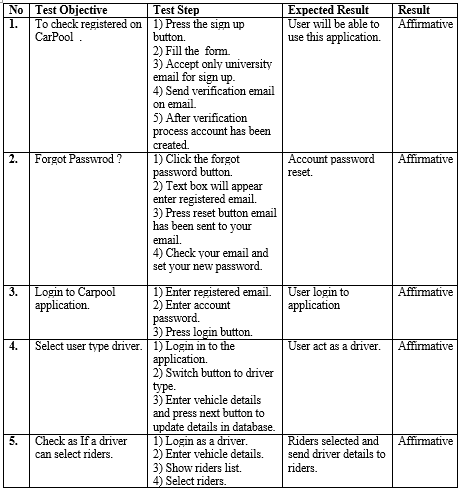
\includegraphics[width=0.8\textwidth]{UsabilityTesting1}
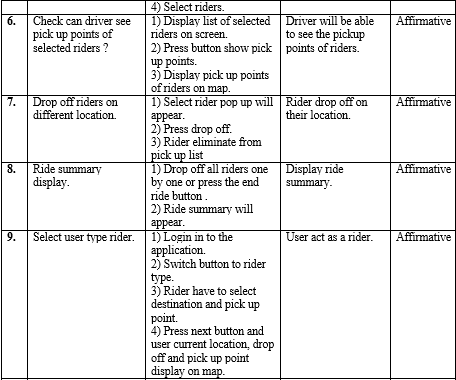
\includegraphics[width=0.8\textwidth]{UsabilityTesting2}
\captionof{table}{Usability Testing}
\end{figure}

\begin{figure}
\centering
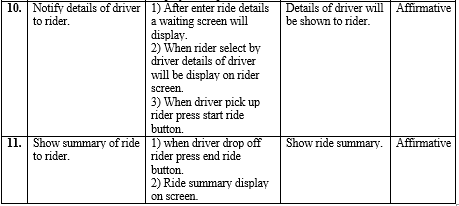
\includegraphics[width=0.8\textwidth]{UsabilityTesting3}
\end{figure}

\begin{figure}
\section{Software performance testing}
\subsubsection{user interface testing}
\centering
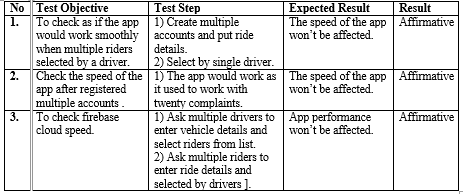
\includegraphics[width=0.8\textwidth]{PFTesting}
\captionof{table}{Software Performance Testing}
\end{figure}

\begin{figure}
\section{Compatibility testing}
\subsubsection{Compatibility testing}
\centering
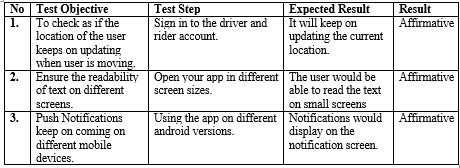
\includegraphics[width=0.8\textwidth]{CompatibilityTesting}
\captionof{table}{Compatibility testing}
\end{figure}

\begin{figure}
\section{Exception handling}
\subsubsection{Exception handling}
\centering
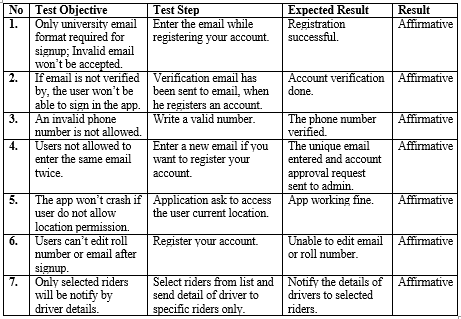
\includegraphics[width=0.8\textwidth]{EHTesting}
\captionof{table}{Exception Handling}
\end{figure}

\begin{figure}
\section{Security testing}
\subsubsection{Security testing}
\centering
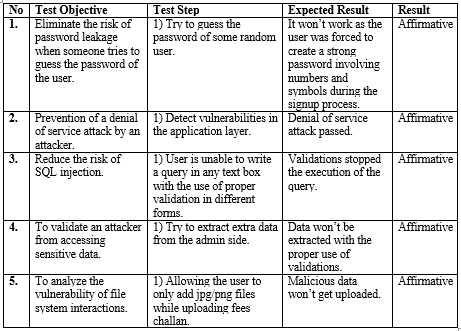
\includegraphics[width=0.8\textwidth]{SecurityTesting}
\captionof{table}{Security Testing}
\end{figure}

\begin{figure}[t]
\section{Installation testing}
\subsubsection{Installation testing}
\centering
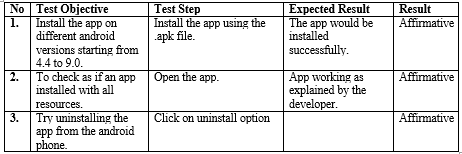
\includegraphics[width=0.8\textwidth]{InstallationTesting}
\captionof{table}{Installation Testing}
\end{figure}


